\documentclass[11pt,a4paper]{article}

% Permite compilar tanto de dentro de Artefatos/ quanto da raiz do projeto no Oleafly
\IfFileExists{config/packages.tex}{\def\artefatosdir{}}{\def\artefatosdir{Artefatos/}}
\makeatletter
\edef\input@path{{\artefatosdir}}
\makeatother

\usepackage[utf8]{inputenc}
\usepackage[T1]{fontenc}
\usepackage{listings}
\usepackage{lmodern}
\usepackage[portuguese]{babel}
\usepackage{graphicx}
\usepackage{amsmath}
\usepackage{amsfonts}
\usepackage{amssymb}
\usepackage{float}
\usepackage{caption}
\usepackage{subcaption}
\usepackage{xcolor}
\usepackage{colortbl}
\usepackage{fancyhdr}
\usepackage{geometry}
\usepackage{titlesec}
\usepackage{lipsum}
% O hyperref precisa vir antes do abntex2cite, senão sobrescreve o \bibitem dele
\usepackage[hidelinks]{hyperref}
\usepackage[alf]{abntex2cite}
\usepackage{booktabs}
\usepackage{array}
\usepackage{enumitem}
\usepackage{pdflscape}
\usepackage{tikz}
\usepackage{float}
\usetikzlibrary{trees}

\definecolor{headercolor}{HTML}{b11116}
\definecolor{secondarycolor}{HTML}{3a5461}

\geometry{
    a4paper,
    top=2.8cm,
    bottom=2.5cm,
    left=2.5cm,
    right=2.5cm,
    headheight=1.2cm,
    headsep=0.5cm
}

\pagestyle{fancy}
\fancyhf{}
\renewcommand{\headrulewidth}{0pt}
\renewcommand{\footrulewidth}{0.5pt}

\fancyhead[L]{%
    \begin{tikzpicture}[remember picture, overlay]
        \fill[headercolor] (current page.north west) rectangle ([yshift=-1.2cm]current page.north east);
        \node[anchor=west, inner sep=0pt] at ([xshift=1cm, yshift=-0.6cm]current page.north west)
            {
\includegraphics[height=0.8cm]{imgs/base/fatec-rgt.png}};
        \node[anchor=east, inner sep=0pt] at ([xshift=-1cm, yshift=-0.6cm]current page.north east)
            {
\includegraphics[height=0.9cm]{imgs/base/cps-logo.png}};
        \node[anchor=east, inner sep=0pt] at ([xshift=-2.8cm, yshift=-0.6cm]current page.north east)
            {
\includegraphics[height=1.05cm]{imgs/base/governo-sp-secretaria-logo.png}};
    \end{tikzpicture}
}

\fancyfoot[L]{\footnotesize\textcolor{secondarycolor}{Faculdade de Tecnologia do Estado de São Paulo\\ fatecregistro.cps.sp.gov.br}}
\fancyfoot[R]{\thepage}

\titleformat{\section}
    {\normalfont\large\bfseries\color{secondarycolor}}
    {\thesection}{1em}{}

\titleformat{\subsection}
    {\normalfont\normalsize\bfseries\color{secondarycolor}}
    {\thesubsection}{1em}{}

% Arquivo reservado para comandos reutilizáveis do documento.


% O abntex2cite só configura a bibliografia se o estilo for definido no preâmbulo
\bibliographystyle{abntex2-alf}

\begin{document}

\begin{titlepage}
    \centering

    \begin{tikzpicture}[remember picture, overlay]
        \fill[headercolor] (current page.north west) rectangle ([yshift=-1.2cm]current page.north east);
        \node[anchor=west, inner sep=0pt] at ([xshift=1cm, yshift=-0.6cm]current page.north west)
            {
\includegraphics[height=0.8cm]{imgs/base/fatec-rgt.png}};
        \node[anchor=east, inner sep=0pt] at ([xshift=-1cm, yshift=-0.6cm]current page.north east)
            {
\includegraphics[height=0.9cm]{imgs/base/cps-logo.png}};
        \node[anchor=east, inner sep=0pt] at ([xshift=-2.8cm, yshift=-0.6cm]current page.north east)
            {
\includegraphics[height=1.05cm]{imgs/base/governo-sp-secretaria-logo.png}};
    \end{tikzpicture}

    \vspace*{3.5cm}

    {\normalsize FACULDADE DE TECNOLOGIA DO ESTADO DE SÃO PAULO\par}
    \vspace{0.5cm}
    {\normalsize DESENVOLVIMENTO DE SOFTWARE MULTIPLATAFORMA\par}

    \vspace{4cm}

    {\normalsize ARTEFATOS DO PROJETO DE SOFTWARE\par}
    \vspace{0.3cm}
    {\normalsize Plataforma de Monitoramento da Etapa de Mosturação na Fabricação de Cerveja Artesanal\par}

    \vspace{3cm}

    {\normalsize
    Haimon Cugler Vieira\\
    João Alexandre Pinto Camargo\\
    Jocieli Pontes Domingues da Silva\\
    Kevin da Silva Oliveira
    }

    \vfill

    {\small Registro -- SP\\
    2026}
\end{titlepage}


\pagestyle{fancy}

\tableofcontents
\newpage


% Diário de Bordo primeiro, como no mapa do PI; depois a ordem do template: Canvas, SWOT, UX/UI, Website, UML, banco de dados e DevOps
\section{Diário de Bordo}

O acompanhamento das atividades do semestre foi feito com um quadro Kanban no GitHub Projects, disponível em \url{https://github.com/orgs/conloq/projects/2}. Cada tarefa é uma \textit{issue} que percorre as colunas Backlog, Ready, In progress, In review, Test e Done, com a sprint, a prioridade, o tamanho e os \textit{story points} registrados no próprio cartão. A Figura~\ref{fig:kanban} mostra o quadro na reta final do semestre.

\begin{figure}[H]
\centering
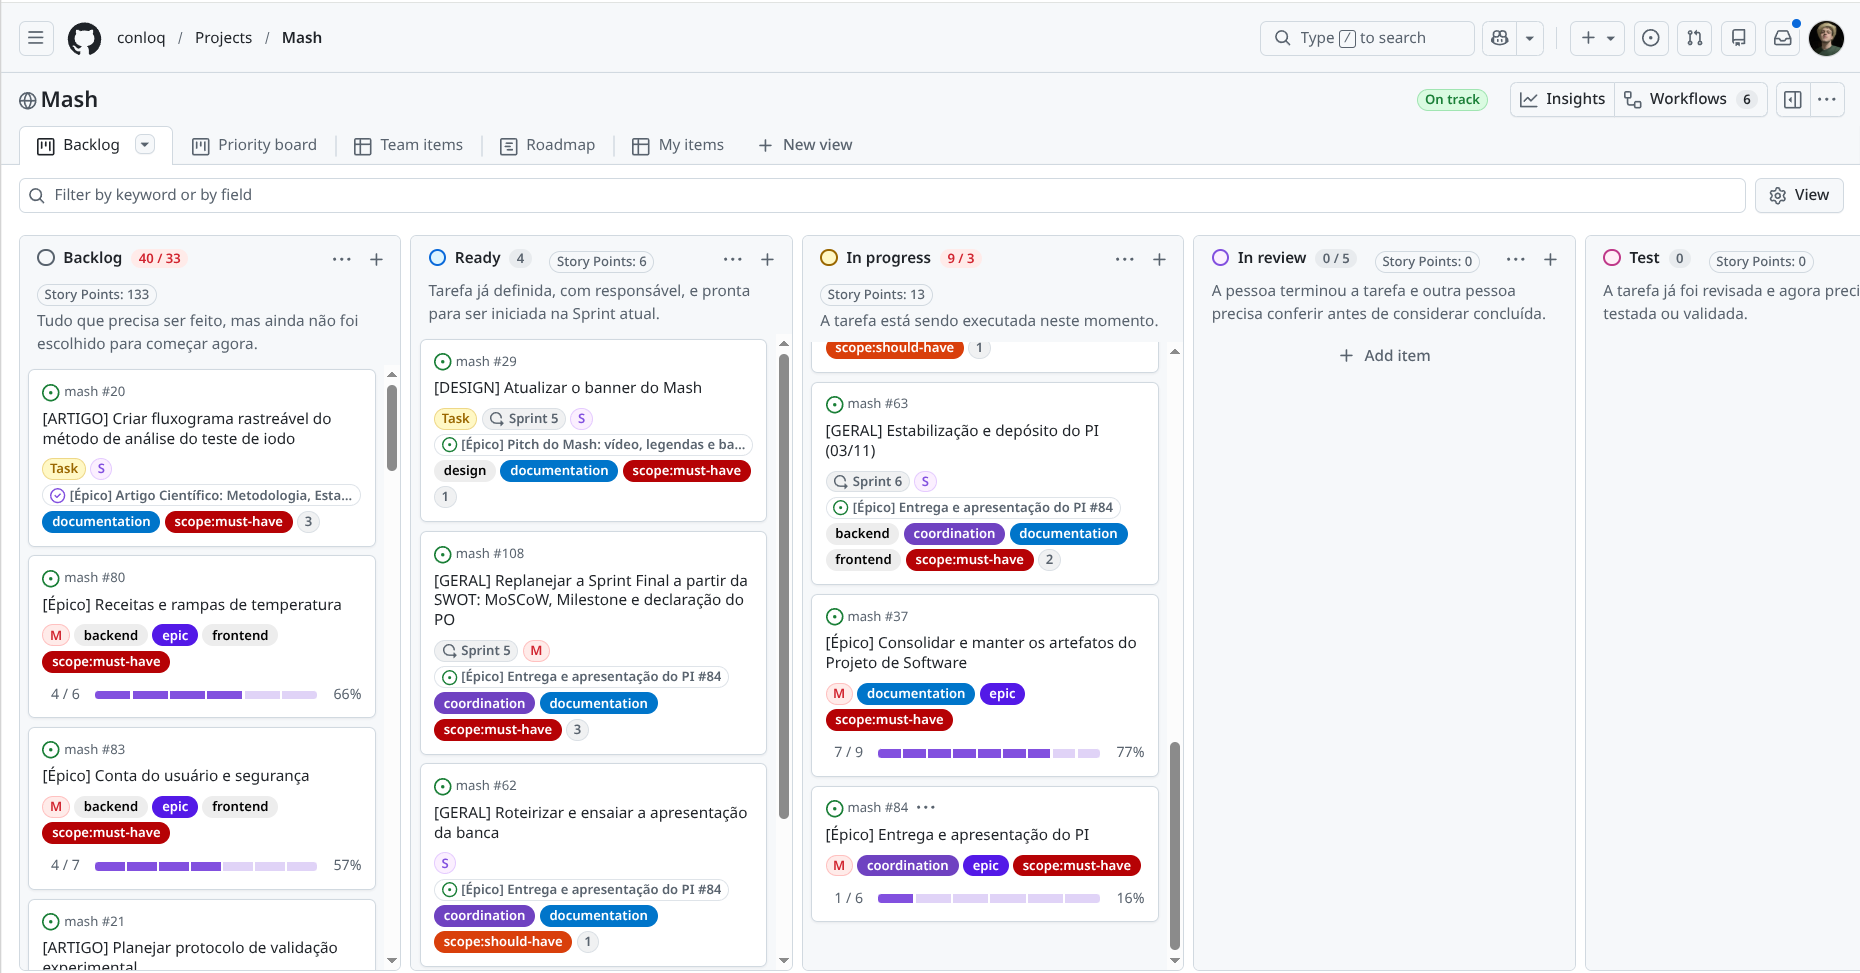
\includegraphics[width=\textwidth]{imgs/kanban.png}
\caption{Quadro Kanban do projeto no GitHub Projects}
\label{fig:kanban}
\end{figure}

O registro das atividades de cada sprint é gerado a partir dos \textit{commits} e das \textit{issues} dos repositórios da equipe e fica publicado em \url{https://github.com/conloq/logbook-backup/tree/main/diario-de-bordo}, com um arquivo por período.

\section{CANVAS: Modelo de Negócio e Estratégia}

O Business Model Canvas~\cite{osterwalder2010} é uma ferramenta visual estratégica\footnote{O Canvas foi desenvolvido por Alexander Osterwalder e é amplamente utilizado em startups e empresas estabelecidas para modelagem de negócios.} que permite descrever, analisar e projetar modelos de negócio de forma clara e objetiva. O canvas é dividido em nove blocos fundamentais que cobrem as principais áreas de um negócio.

\begin{figure}[H]
\centering
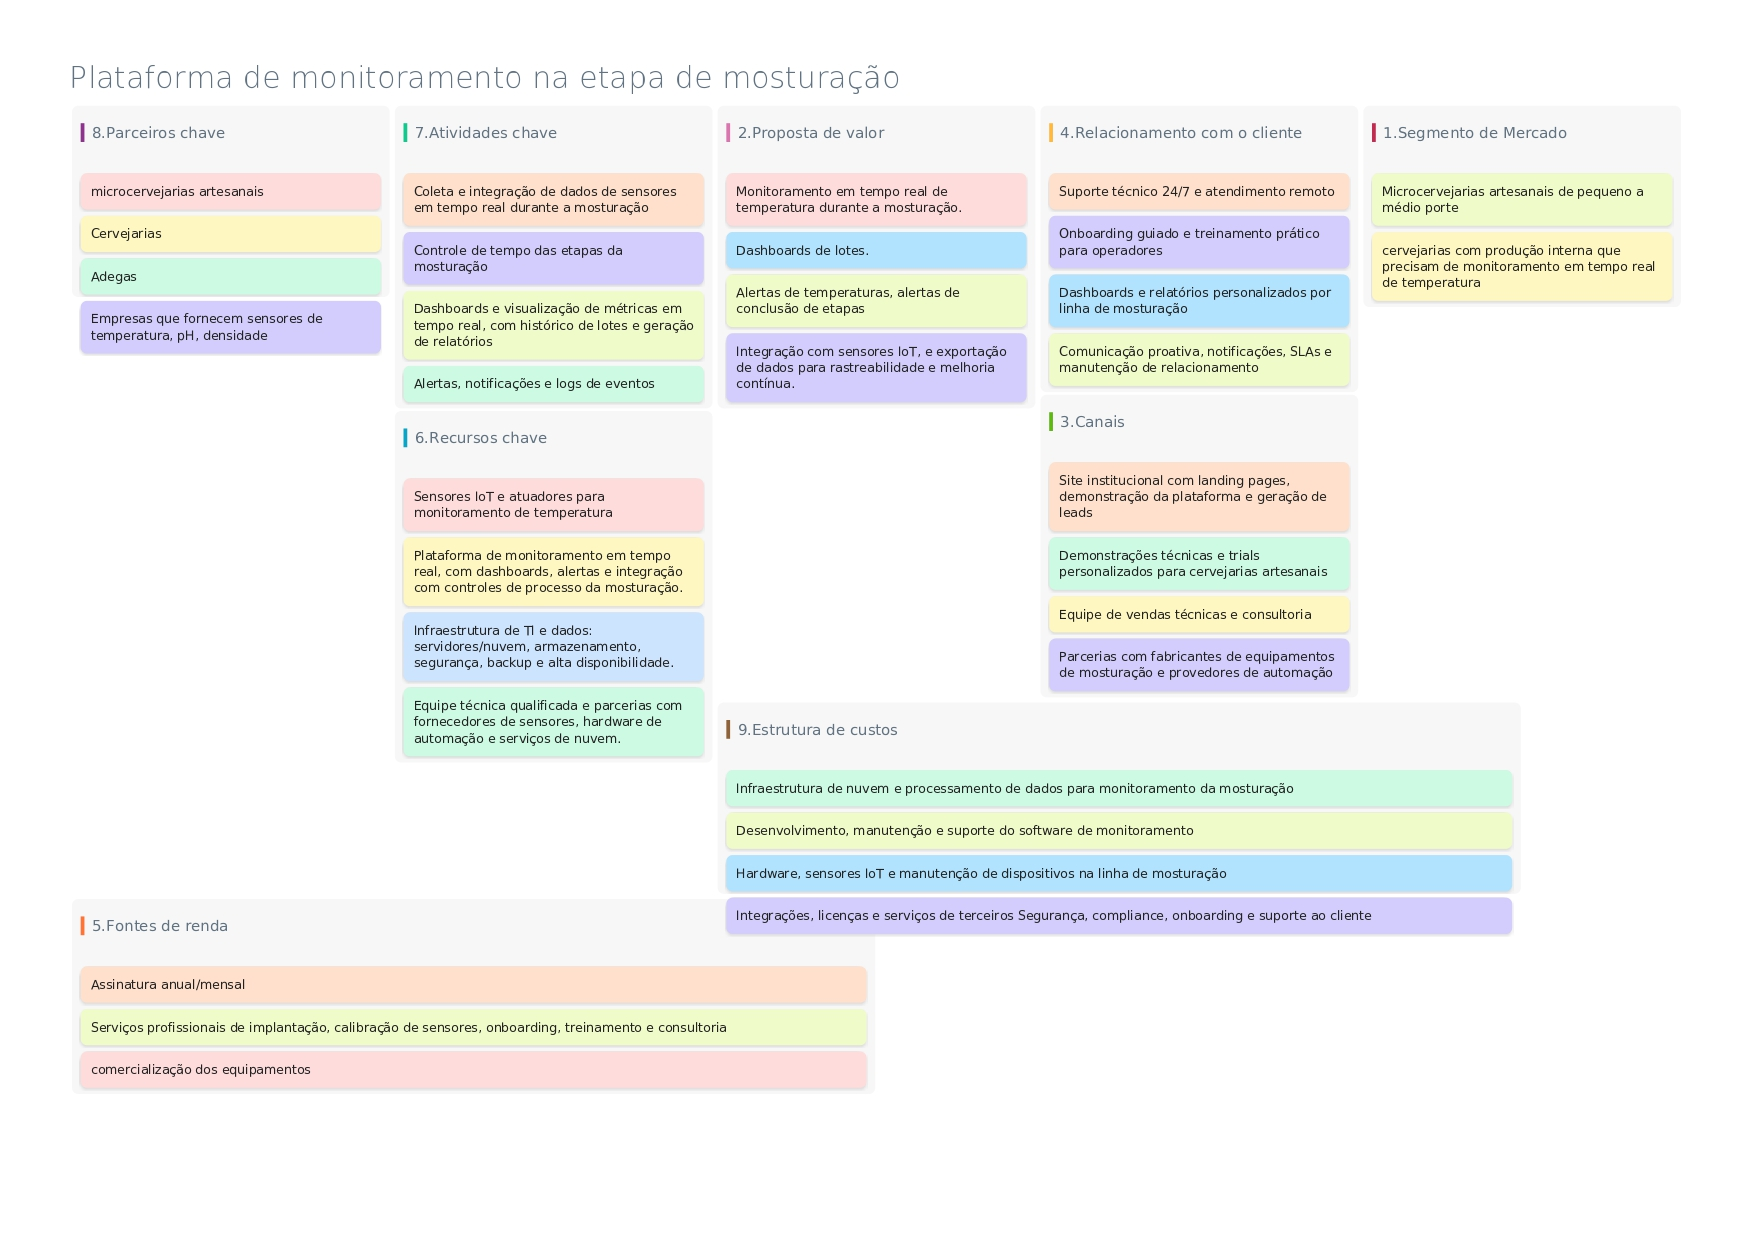
\includegraphics[width=1.1\linewidth]{imgs/canvas.jpg}
\caption{Canvas}
\label{fig:canvas}
\end{figure}

\section{SWOT}

A Análise SWOT\footnote{Também conhecida no Brasil pela sigla FOFA (Forças, Oportunidades, Fraquezas e Ameaças), a ferramenta foi desenvolvida no âmbito da administração estratégica para apoiar o planejamento corporativo e a tomada de decisão.} é uma metodologia de diagnóstico estratégico utilizada para avaliar os ambientes interno e externo de uma organização, projeto ou produto. A ferramenta estrutura-se em uma matriz quadripartida que correlaciona os pontos fortes e fracos inerentes à estrutura interna aos fatores de oportunidades e ameaças provenientes do ecossistema externo~\cite{helms2010}.

A Tabela~\ref{tab:swot} apresenta a análise do Mash na reta final do semestre. Os dados de mercado e técnicos vêm acompanhados da referência que os sustenta.

\newcommand{\swotitem}[1]{\item #1}
\newcommand{\swotcab}[2]{\cellcolor[HTML]{#1}\textbf{#2}}

\begin{table}[H]
\centering
\caption{Análise SWOT do Projeto}
\label{tab:swot}
\renewcommand{\arraystretch}{1.2}
\begin{tabular}{|p{0.46\textwidth}|p{0.46\textwidth}|}
\hline
\multicolumn{2}{|c|}{\textbf{FATORES INTERNOS}} \\
\hline
\swotcab{E3F4EA}{FORÇAS (Strengths)} & \swotcab{FDF3D8}{FRAQUEZAS (Weaknesses)} \\
\hline
\begin{itemize}[leftmargin=*, nosep, after=\vspace{-\baselineskip}]
\swotitem{API com autenticação JWT, senhas guardadas com hash Argon2 e isolamento entre usuários}
\swotitem{Receitas, rampas de temperatura e lotes ligados da tela ao banco de dados}
\swotitem{Schema do banco criado por \textit{migrations} versionadas}
\swotitem{API e frontend publicados em ambiente de nuvem}
\swotitem{Decisões e recorte do semestre registrados em um só lugar}
\end{itemize}
&
\begin{itemize}[leftmargin=*, nosep, after=\vspace{-\baselineskip}]
\swotitem{Sem testes automatizados; a validação é manual, por exceção registrada}
\swotitem{Classificação automática do teste do iodo não implementada; neste semestre o teste é uma simulação na interface}
\swotitem{Equipe de quatro integrantes, com dois dedicados à programação}
\end{itemize}
\\
\hline
\multicolumn{2}{|c|}{\textbf{FATORES EXTERNOS}} \\
\hline
\swotcab{E5F0F8}{OPORTUNIDADES (Opportunities)} & \swotcab{FDECEA}{AMEAÇAS (Threats)} \\
\hline
\begin{itemize}[leftmargin=*, nosep, after=\vspace{-\baselineskip}]
\swotitem{1.949 cervejarias registradas no Brasil, com crescimento de 5,5\% em 2024 \cite{MAPA2025}}
\swotitem{EXPOBEER Vale do Ribeira e a produção regional de cerveja artesanal \cite{ExpoBeerEvento2025}}
\swotitem{A banca avalia o fluxo principal demonstrado, e não funcionalidades fora do recorte}
\end{itemize}
&
\begin{itemize}[leftmargin=*, nosep, after=\vspace{-\baselineskip}]
\swotitem{Prazo do depósito do projeto em 03/11/2026}
\swotitem{O plano gratuito do Render desliga a API após 15 minutos sem uso, e ela leva cerca de 1 minuto para voltar}
\swotitem{A iluminação do ambiente altera a leitura da cor do iodo \cite{li2025starch}}
\end{itemize}
\\
\hline
\end{tabular}
\end{table}

\subsection{Recomendações Estratégicas}

Com base na análise SWOT, a equipe definiu as estratégias da reta final:

\begin{itemize}
\item \textbf{Forças + Oportunidades:} demonstrar o ciclo completo, do login ao lote, com usuário, receita e lote já cadastrados.
\item \textbf{Fraquezas + Oportunidades:} congelar o escopo e executar na véspera um roteiro de validação manual do fluxo principal.
\item \textbf{Forças + Ameaças:} manter um ambiente local com as \textit{migrations} aplicadas e os dados de demonstração, e gravar um vídeo do fluxo como plano B.
\item \textbf{Fraquezas + Ameaças:} retirar do semestre o teste do iodo automatizado e apresentar a simulação de interface já pronta.
\end{itemize}

\section{UX/UI: Design de Interface e Experiência do Usuário}

O design UX/UI da plataforma foi desenvolvido com o objetivo de proporcionar uma interface intuitiva, organizada e de fácil utilização para os produtores de cerveja artesanal durante o acompanhamento do processo de mosturação e realização do teste do iodo.

As telas foram desenvolvidas utilizando prototipação no Figma, permitindo simular o fluxo completo da aplicação antes da implementação do sistema.

A construção da interface priorizou simplicidade operacional, contraste visual e facilidade de navegação, permitindo que o usuário consiga acessar rapidamente as principais funcionalidades da plataforma durante o processo produtivo.

\subsection{Guia de Estilos}

A identidade visual da plataforma foi desenvolvida utilizando cores inspiradas no processo cervejeiro e em interfaces modernas de aplicações web, buscando transmitir organização, contraste visual e facilidade de navegação para o usuário.

A composição visual segue a proporção 60-30-10, técnica amplamente utilizada no design de interfaces para criar equilíbrio visual entre elementos estruturais, componentes secundários e elementos de destaque.

\begin{table}[H]
\centering
\caption{Identidade Visual da Plataforma}
\label{tab:cores}
\begin{tabular}{|l|c|l|p{6cm}|}
\hline
\textbf{Cor} & \textbf{Proporção} & \textbf{Código HEX} & \textbf{Aplicação} \\
\hline

\colorbox[HTML]{FAFAFA}{\rule{0pt}{0.4cm}\hspace{1cm}} &
60\% &
\#FAFAFA &
Cor estrutural da identidade visual, utilizada nos fundos principais da interface e áreas de respiro visual. \\
\hline

\colorbox[HTML]{4E342E}{\rule{0pt}{0.4cm}\hspace{1cm}} &
30\% &
\#4E342E &
Cor secundária aplicada no cabeçalho, menus e fundos secundários da plataforma. \\
\hline

\colorbox[HTML]{F57C00}{\rule{0pt}{0.4cm}\hspace{1cm}} &
10\% &
\#F57C00 &
Cor de destaque utilizada em botões principais, links e chamadas de ação da interface. \\
\hline

\colorbox[HTML]{000000}{\rule{0pt}{0.4cm}\hspace{1cm}} &
-- &
\#000000 &
Cor utilizada para textos principais e elementos informativos da interface. \\
\hline

\end{tabular}
\end{table}

\subsection{Tipografia}

A tipografia da plataforma foi definida com o objetivo de garantir boa legibilidade, organização visual e identidade moderna para a interface do sistema.

As fontes selecionadas foram escolhidas considerando acessibilidade, clareza na leitura e adaptação para diferentes tamanhos de tela.

\begin{itemize}

\item \textbf{Poppins}

Fonte moderna e versátil, utilizada em títulos, chamadas e elementos de destaque da interface. Seus traços suaves e equilibrados transmitem inovação, dinamismo e proximidade visual, contribuindo para uma identidade moderna da plataforma.

\item \textbf{Roboto}

Fonte neutra e altamente legível, utilizada em textos longos e no corpo do conteúdo da aplicação. Sua estrutura proporciona clareza visual e facilidade de leitura em diferentes resoluções e tamanhos de tela.

\end{itemize}
\section{Website: Estrutura e Especificações Técnicas Web}

Esta seção documenta a landing page da equipe. O website foi desenvolvido com o objetivo de apresentar os integrantes da equipe, divulgar o projeto integrador e disponibilizar informações institucionais e de contato.

\subsection{Mapa do Site da Equipe} O mapa do site (sitemap) mostra a hierarquia e organização das páginas do website da equipe:
\begin{figure}[H]
\centering
\begin{tikzpicture}[
    level 1/.style={
        sibling distance=4cm,
        level distance=1.8cm
    },
    level 2/.style={
        sibling distance=2.5cm,
        level distance=1.8cm
    },
    every node/.style={
        rectangle,
        draw,
        rounded corners,
        fill=brown!20,
        text width=2.8cm,
        align=center,
        font=\small,
        minimum height=0.9cm
    }
]

\node {Conloq}
    child {
        node {Sobre Nós}
            child { node {Objetivo} }
            child { node {Propósitos} }
    }
    child {
        node {Equipe}
            child { node {Integrantes} }
    }
    child {
        node {Portfólio}
            child { node {Projetos} }
    }
    child {
        node {Contato}
            child { node {Redes Sociais} }
            child { node {Contatos} }
    };
\end{tikzpicture}
\caption{Estrutura de navegação}
\label{fig:sitemap}
\end{figure}

\textbf{Principais seções da landing page da equipe:}

\begin{itemize}

    \item \textbf{Conloq:} Apresentação inicial da equipe e destaque do projeto desenvolvido.

    \item \textbf{Sobre Nós:} Informações sobre a equipe, objetivos e proposta do projeto.

    \item \textbf{Equipe:} Apresentação dos integrantes responsáveis pelo desenvolvimento da plataforma, incluindo nome, função e tecnologias utilizadas.

    \item \textbf{Portfólio:} Exibição dos projetos, tecnologias e soluções desenvolvidas pela equipe.

    \item \textbf{Contato:} Área destinada às informações de comunicação da equipe, contendo links para redes sociais, GitHub, LinkedIn, e-mail e demais canais de contato.

\end{itemize}

\subsection{Especificações Técnicas do Site da Equipe}

\begin{table}[H]
\centering
\caption{Stack Tecnológica}
\label{tab:stack-web}
\begin{tabular}{|l|l|p{6cm}|}
\hline
\textbf{Camada} & \textbf{Tecnologia} & \textbf{Descrição} \\
\hline
Estrutura & HTML5 & Utilizado para estruturar as páginas da landing page \\
\hline
Estilização & CSS3 & Estilização e organização visual da interface \\
\hline
Interatividade & JavaScript & Funcionalidades e interações da página \\
\hline
Responsividade & CSS & Interface para desktop e dispositivos móveis \\
\hline
Hospedagem & GitHub Pages & Deploy e hospedagem do website \\
\hline
Versionamento & Git e GitHub & Gerenciamento e versionamento do código-fonte \\
\hline
\end{tabular}
\end{table}
\section{Diagramas UML: Modelagem Visual do Sistema}

\subsection{Diagrama de Casos de Uso}

O diagrama de casos de uso representa as funcionalidades do sistema do ponto de vista do usuário, demonstrando as interações entre os atores e os principais recursos disponíveis na plataforma.

\begin{figure}[H]
\centering
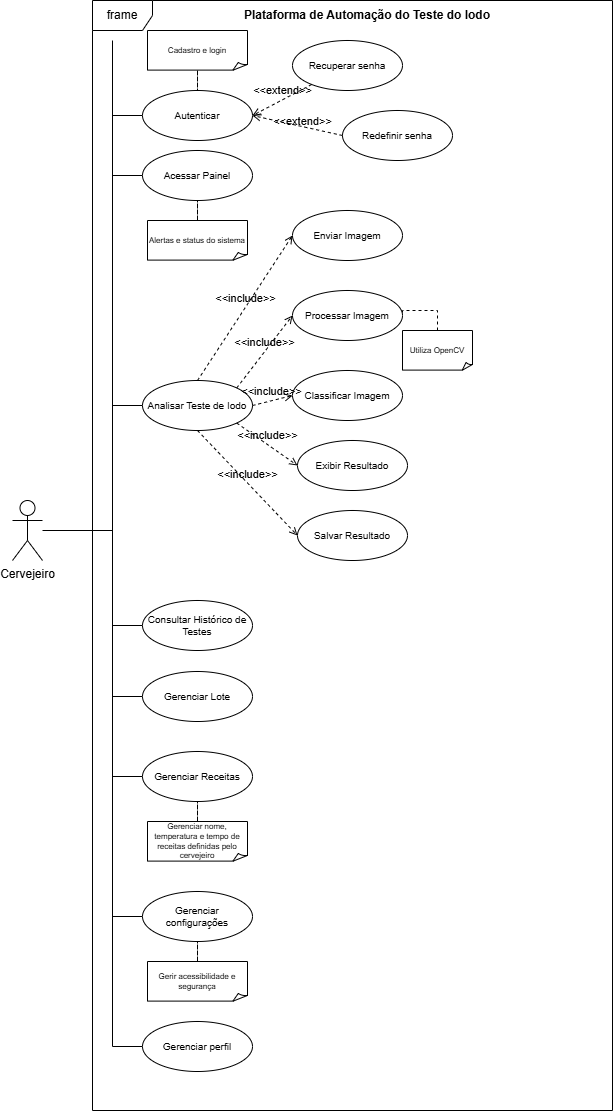
\includegraphics[height=0.9\textheight, keepaspectratio]{imgs/caso-de-uso.png}
\caption{Diagrama de Casos de Uso}
\label{fig:caso-de-uso}
\end{figure}

\subsection{Diagrama de Classes}

O diagrama de classes mostra a estrutura estática do sistema:

\begin{figure}[H]
\centering
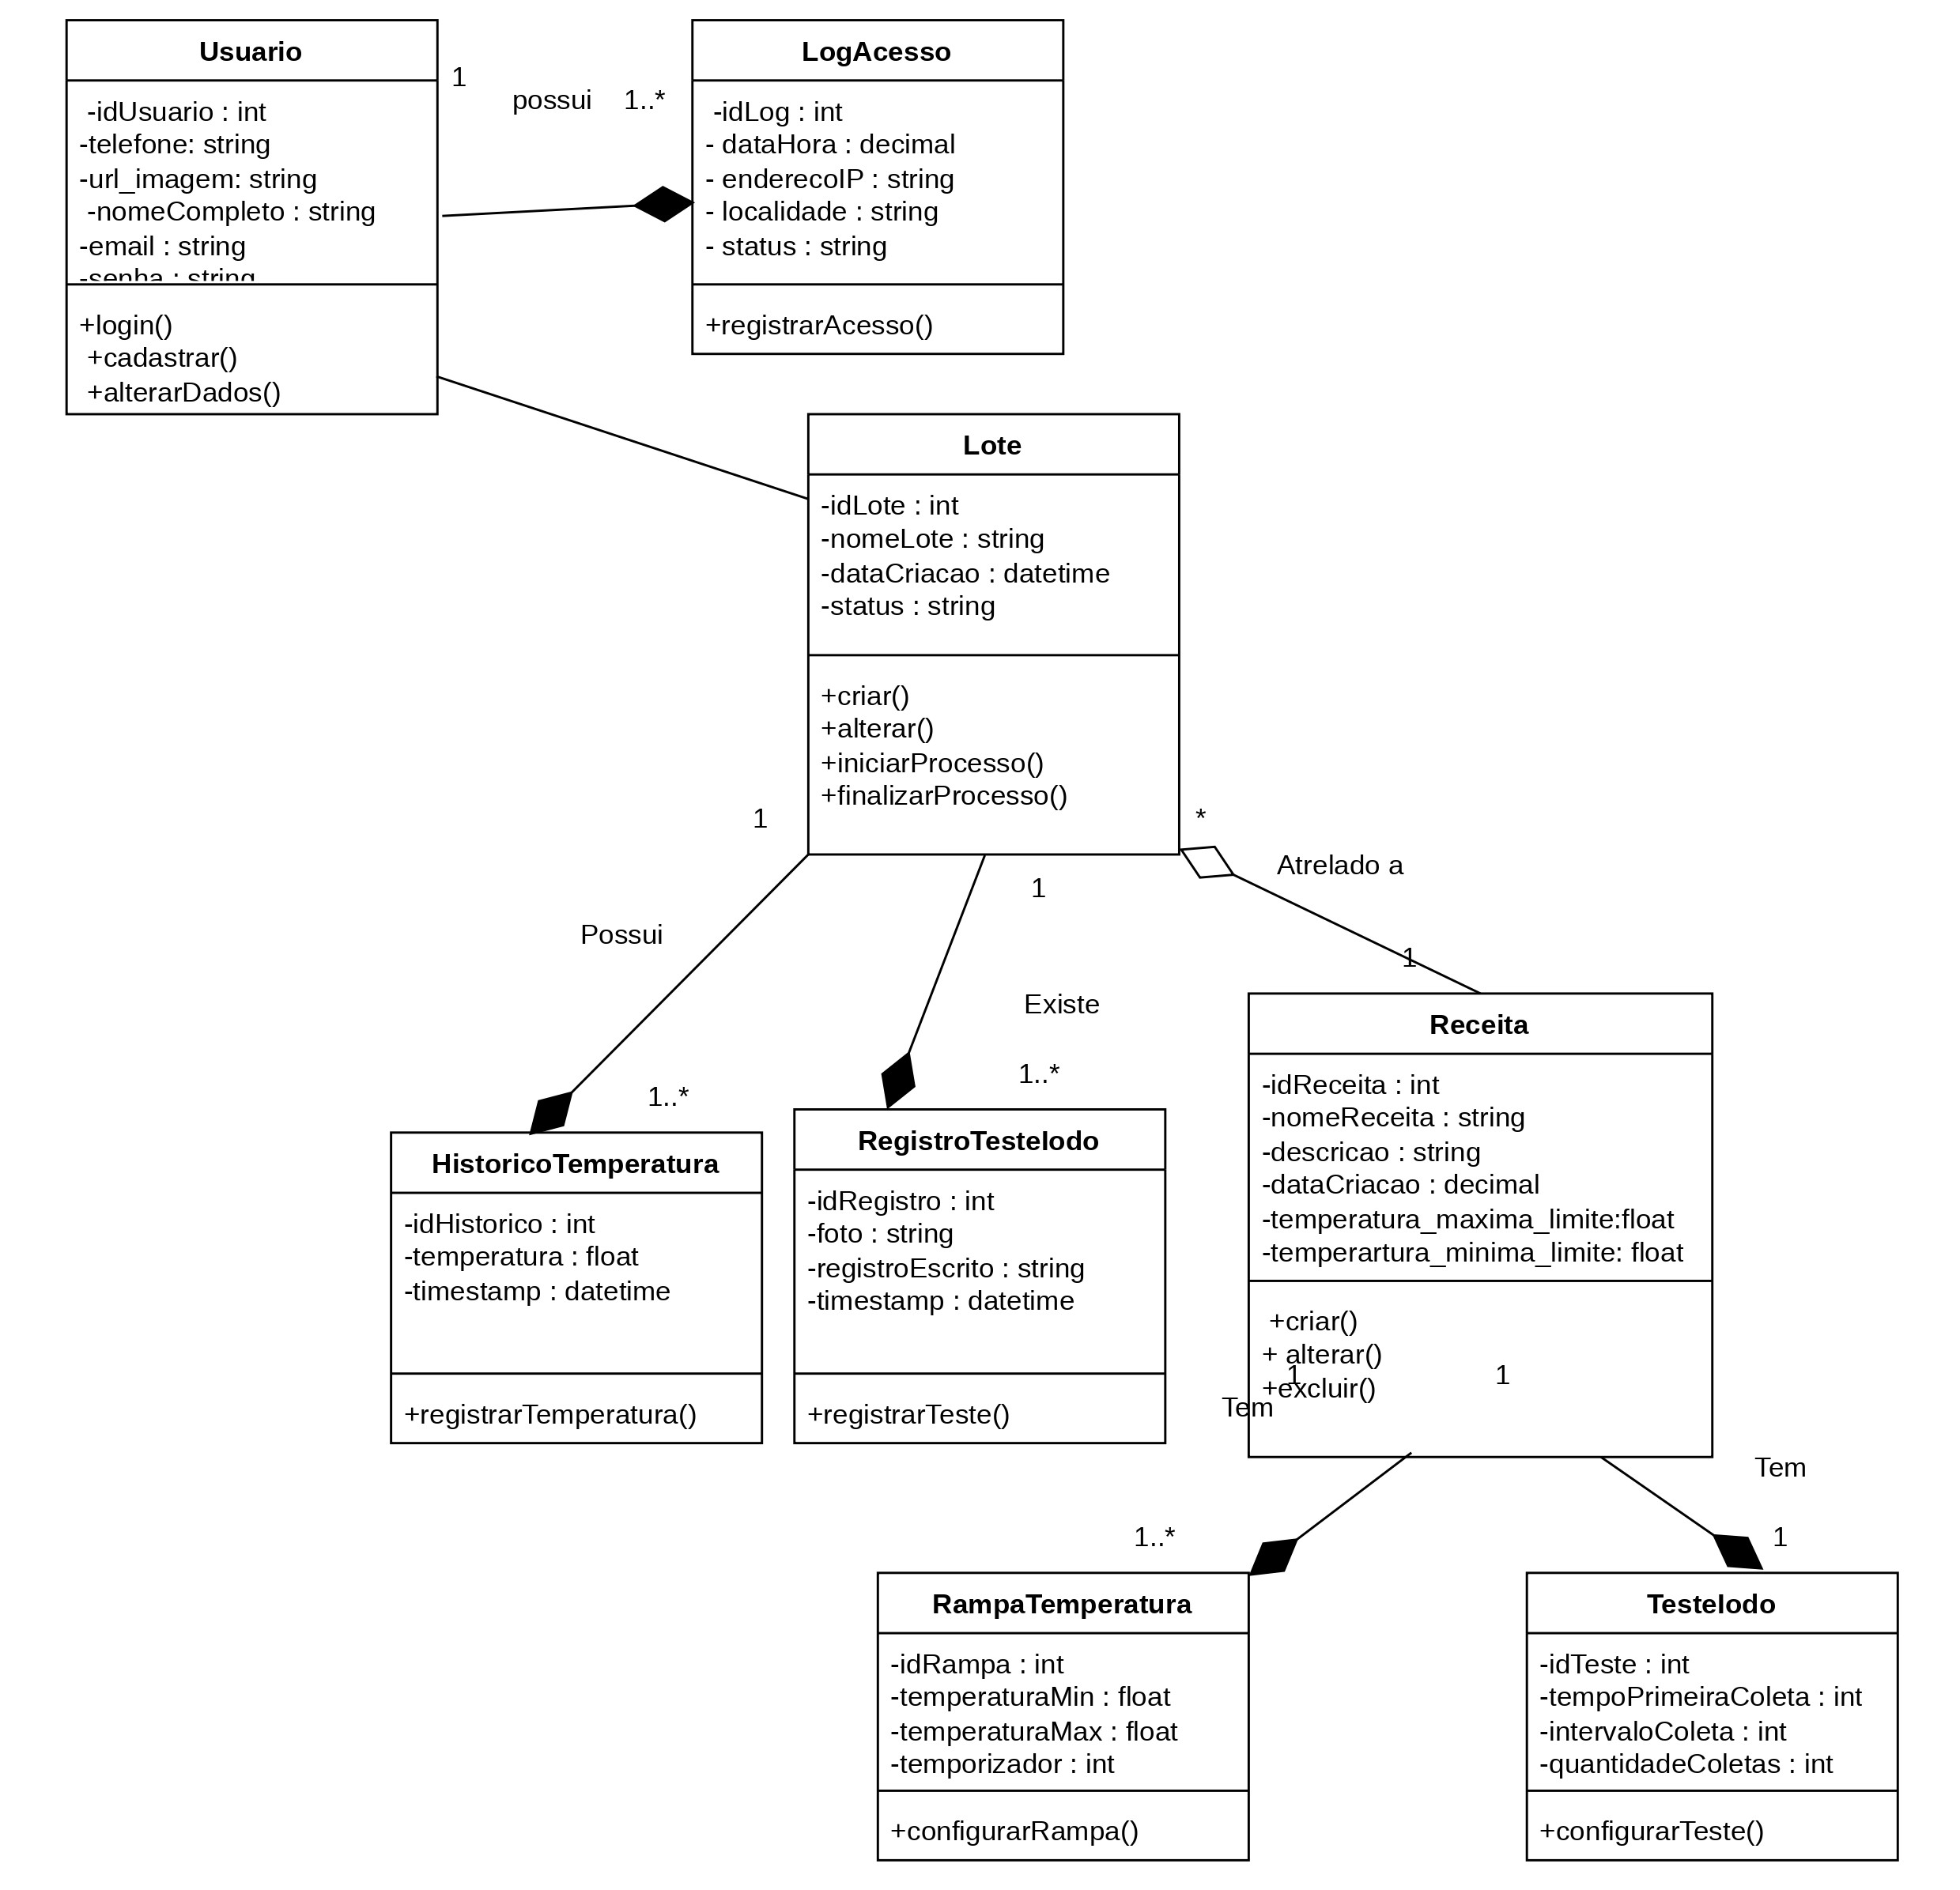
\includegraphics[width=\textwidth]{imgs/diagrama-de-classes.jpg}
\caption{Diagrama de Classes}
\label{fig:diagrama-de-classes}
\end{figure}

\subsection{Diagrama de Objetos}

O diagrama de objetos representa instâncias reais das classes utilizadas no sistema em um determinado momento da execução da aplicação. O diagrama de objetos demonstra exemplos concretos dos dados manipulados pela plataforma.

\begin{figure}[H]
\centering
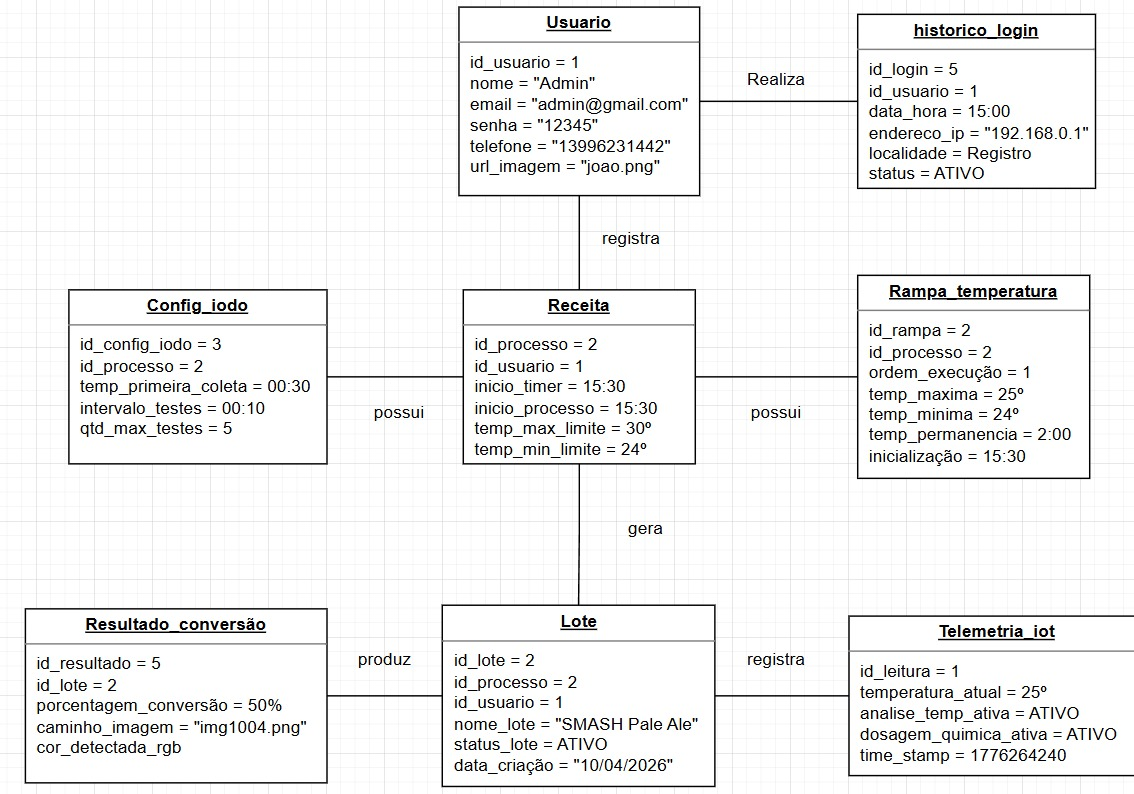
\includegraphics[width=0.9\linewidth]{imgs/diagrama-de-objetos.jpeg}
\caption{Diagrama de Objetos}
\label{fig:diagrama-objetos}
\end{figure}
\section{Diagrama de Banco de Dados}

\subsection{Modelo Entidade-Relacionamento (MER)}

O Modelo Entidade-Relacionamento (MER)~\cite{chen1976} foi utilizado para representar a estrutura conceitual do banco de dados da plataforma de verificação do teste do iodo. O objetivo desse modelo é demonstrar as entidades presentes no sistema, seus atributos e os relacionamentos existentes entre elas.

\begin{figure}[H]
\centering
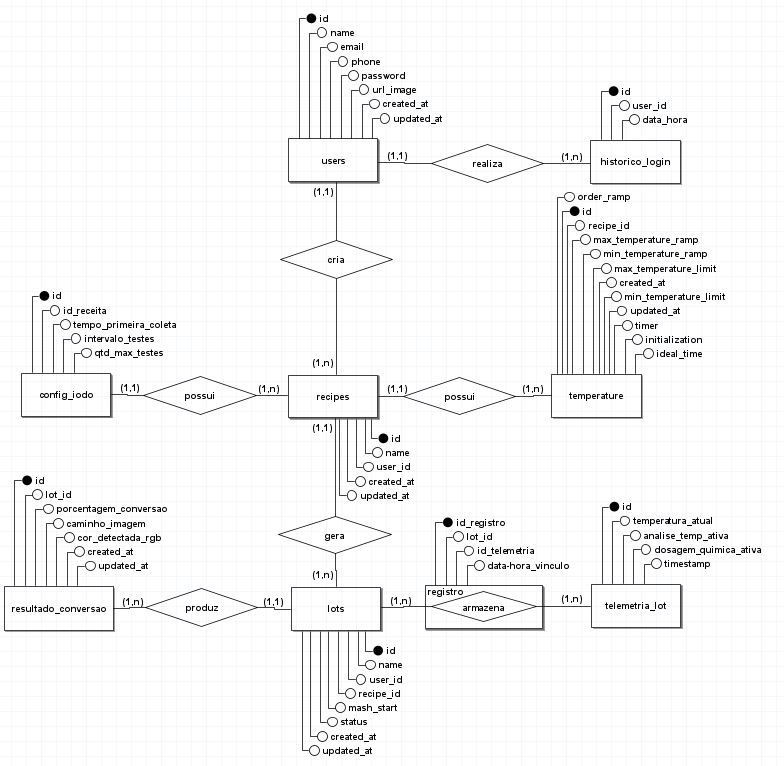
\includegraphics[width=0.9\linewidth]{imgs/diagrama-mer.png}
\caption{Modelo Entidade-Relacionamento}
\label{fig:diagrama-de-banco-de-dados}
\end{figure}
\section{DevOps: Infraestrutura}

\subsection{Introdução}

A infraestrutura de rede apresentada foi desenvolvida para atender às necessidades de comunicação e gerenciamento da plataforma de verificação do teste do iodo por visão computacional aplicada à produção de cerveja artesanal.

A rede é responsável por interligar servidor, computador de monitoramento, dispositivos móveis e equipamentos de comunicação, garantindo estabilidade na transmissão dos dados, armazenamento das análises e acesso à aplicação web. Além disso, a infraestrutura permite comunicação entre os componentes do sistema utilizados durante o processo de mosturação.

\subsection{Topologia da Rede}

A infraestrutura utiliza topologia em estrela, na qual todos os dispositivos estão conectados a um switch central localizado na sala técnica. O switch está ligado ao modem/roteador responsável pelo acesso à internet e funcionamento como gateway padrão da rede. Essa abordagem facilita a manutenção, gerenciamento e expansão futura da infraestrutura.

\subsection{Estrutura da Rede}

A rede cabeada utiliza cabos Ethernet padrão Cat6, proporcionando maior estabilidade e velocidade na transmissão dos dados. O servidor possui endereço IP fixo e é responsável pelo armazenamento e gerenciamento das informações do sistema.

Além da rede cabeada, a infraestrutura também possui suporte à comunicação sem fio por meio de um ponto de acesso Wi-Fi instalado na sala técnica, permitindo conexão de dispositivos móveis utilizados durante o processo de produção e monitoramento da plataforma.

\begin{table}[H]
\centering
\caption{Endereçamento da Rede}
\label{tab:rede}
\begin{tabular}{|l|l|p{6cm}|}
\hline
\textbf{Dispositivo} & \textbf{Endereço IP} & \textbf{Observação} \\
\hline
Roteador / Gateway & 192.168.0.1 & Acesso à internet \\
\hline
Servidor & 192.168.0.2 & Armazenamento de dados \\
\hline
Computador da Sala Técnica & 192.168.0.10 & Monitoramento do sistema \\
\hline
Dispositivos móveis & DHCP automático & Conexão Wi-Fi \\
\hline
\end{tabular}
\end{table}

\subsection{Arquitetura de Rede}

\begin{table}[H]
\centering
\caption{Componentes da Infraestrutura da Rede}
\label{tab:infraestrutura}
\begin{tabular}{|l|p{10cm}|}
\hline
\textbf{Componente} & \textbf{Descrição} \\
\hline

\textbf{Roteador / Gateway} &
\begin{itemize}[leftmargin=*, nosep]
    \item Responsável pelo acesso à internet
    \item Atua como gateway padrão da rede
    \item Distribuição da comunicação da rede local
\end{itemize} \\
\hline

\textbf{Switch Central} &
\begin{itemize}[leftmargin=*, nosep]
    \item Interligação dos dispositivos da rede
    \item Estrutura central da topologia estrela
    \item Facilita expansão e manutenção da infraestrutura
\end{itemize} \\
\hline

\textbf{Servidor} &
\begin{itemize}[leftmargin=*, nosep]
    \item Processamento das análises do sistema
    \item Execução da aplicação Flask
    \item Armazenamento dos dados e resultados
\end{itemize} \\
\hline

\textbf{Computador da Sala Técnica} &
\begin{itemize}[leftmargin=*, nosep]
    \item Monitoramento do sistema
    \item Gerenciamento operacional da plataforma
    \item Controle local da aplicação
\end{itemize} \\
\hline

\textbf{Dispositivos Móveis} &
\begin{itemize}[leftmargin=*, nosep]
    \item Captura das imagens do teste do iodo
    \item Acesso remoto à plataforma
    \item Comunicação via rede Wi-Fi
\end{itemize} \\
\hline

\end{tabular}
\end{table}

\subsection{Diagrama de Infraestrutura}

A Figura \ref{fig:diagrama-de-infraestrutura} apresenta o diagrama da infraestrutura utilizada na plataforma, demonstrando a comunicação entre os dispositivos da rede.

\begin{figure}[H]
\centering
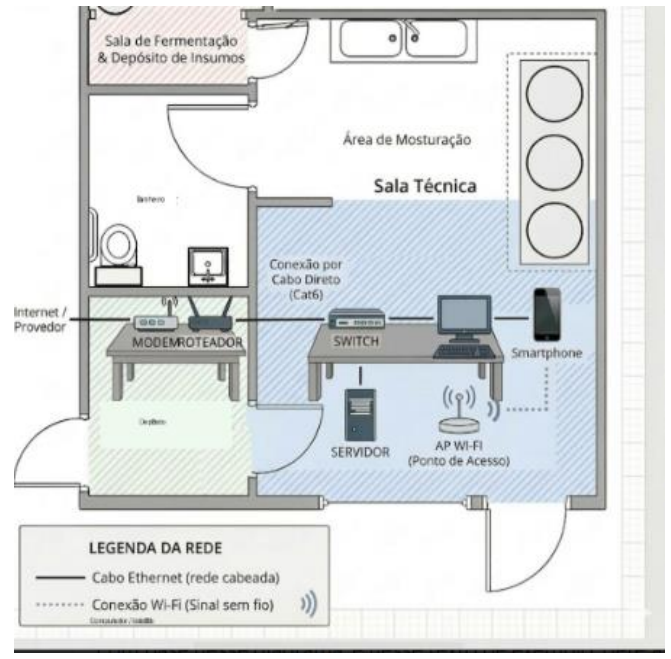
\includegraphics[width=0.9\linewidth]{imgs/redes.png}
\caption{Diagrama de Infraestrutura do Sistema}
\label{fig:diagrama-de-infraestrutura}
\end{figure}

\subsection{Diagrama de Usabilidade}

A Figura \ref{fig:diagrama-de-usabilidade} apresenta o diagrama de usabilidade da plataforma, demonstrando o fluxo de interação entre o funcionário e os principais componentes do sistema. O diagrama evidencia como o usuário acessa a aplicação, envia a imagem do teste do iodo, recebe o resultado da análise e consulta as informações armazenadas.

\begin{figure}[H]
\centering
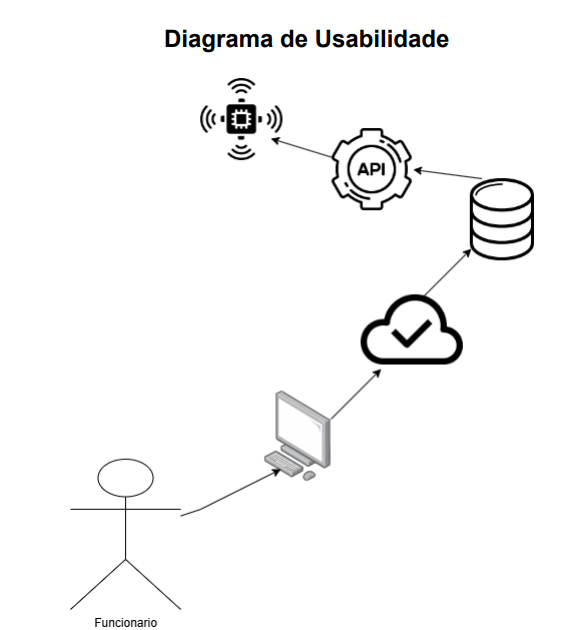
\includegraphics[width=0.9\linewidth]{imgs/usabilidade.png}
\caption{Diagrama de Usabilidade}
\label{fig:diagrama-de-usabilidade}
\end{figure}

\subsection{Conclusão}

A infraestrutura proposta oferece uma solução simples, funcional e segura para o ambiente de produção da cervejaria artesanal. A utilização da topologia em estrela facilita o gerenciamento da rede, melhora a comunicação entre os dispositivos e permite futuras expansões do sistema, incluindo integração com novas soluções de automação e monitoramento.
\newpage
\addcontentsline{toc}{section}{Referências}
\bibliography{\artefatosdir referencias}

\end{document}
